\documentclass{article}
\usepackage{tikz}
\usetikzlibrary{positioning, arrows.meta, shapes.geometric}
\usepackage{amsmath, amssymb}

% 必要なマクロの定義
\newcommand{\lSdti}{$\lambda_{\textrm{S}}^{\textrm{DTI}}$}
\newcommand{\token}[1]{\texttt{#1}}

\begin{document}

\begin{figure}[tb]
    \centering
    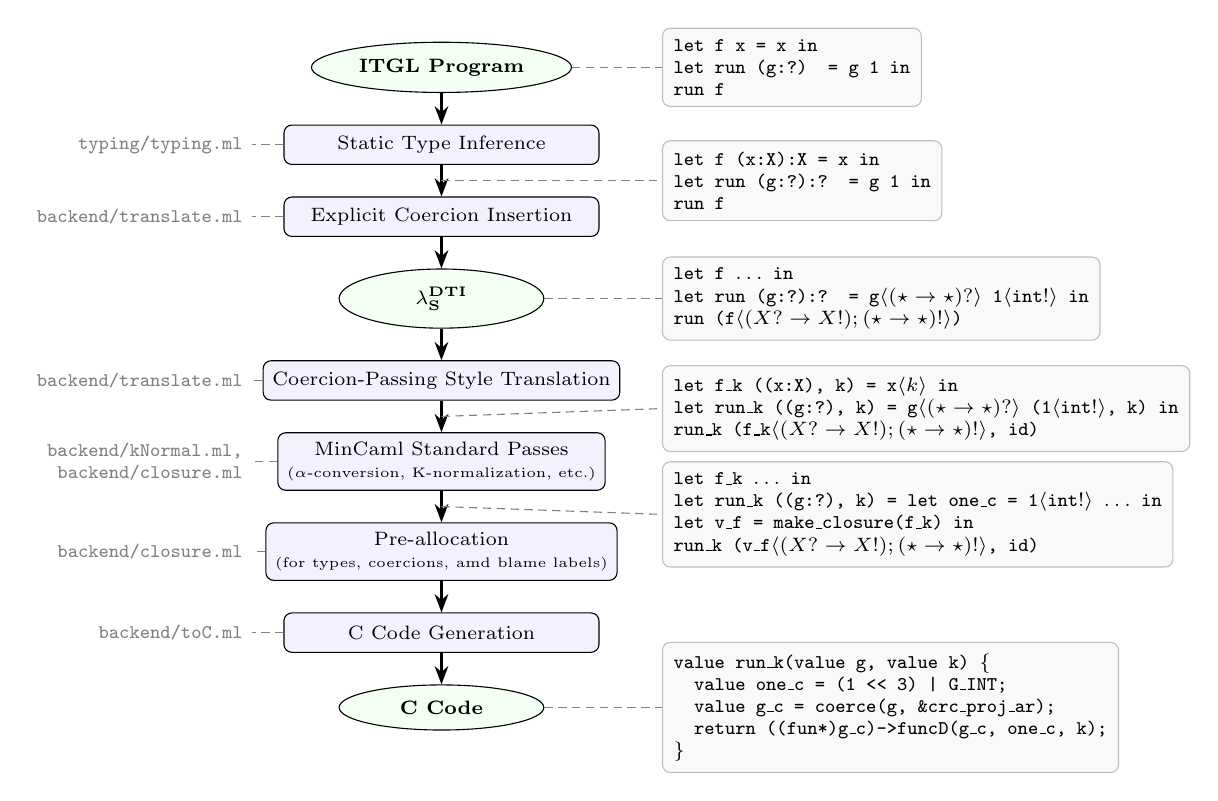
\begin{tikzpicture}[
        node distance=0.4cm and 0.4cm,
        % 変換パス（処理）のスタイル
        pass/.style={rectangle, draw, rounded corners=1mm, minimum width=4.0cm, minimum height=0.5cm, align=center, fill=blue!5, font=\scriptsize},
        % 言語（データ）のスタイル
        lang/.style={ellipse, draw, minimum width=2.6cm, minimum height=0.4cm, align=center, fill=green!5, font=\scriptsize\bfseries},
        % 矢印のスタイル
        arrow/.style={->, >=Stealth, thick},
        % プログラム例のスタイル
        code/.style={rectangle, draw=gray!50, rounded corners=1mm, fill=gray!5, inner sep=4pt, align=left, font=\scriptsize\ttfamily},
        % 左側のファイル名用のスタイル（ここで定義しています）
        file/.style={font=\scriptsize\ttfamily, gray, align=right, anchor=east}
    ]

    % ノードの定義と配置
    \node[lang] (itgl) {ITGL Program};
    \node[pass, below=of itgl] (infer) {Static Type Inference};
    \node[pass, below=of infer] (insert) {Explicit Coercion Insertion};
    \node[lang, below=of insert] (lsdti) {\lSdti};
    \node[pass, below=of lsdti] (cps) {Coercion-Passing Style Translation};
    \node[pass, below=of cps] (mincaml) {MinCaml Standard Passes \\ {\tiny ($\alpha$-conversion, K-normalization, etc.)}};
    \node[pass, below=of mincaml] (allocation) {Pre-allocation \\ {\tiny (for types, coercions, amd blame labels)}};
    % \node[pass, below=of allocation] (idopt) {\textsf{id}-Coercion Dispatch};
    \node[pass, below=of allocation] (codegen) {C Code Generation};
    \node[lang, below=of codegen] (ccode) {C Code};

    % 矢印の描画と中間座標（coordinate）の定義
    \draw[arrow] (itgl) -- coordinate (arr_itgl) (infer);
    \draw[arrow] (infer) -- coordinate (arr_infer) (insert);
    \draw[arrow] (insert) -- coordinate (arr_insert) (lsdti);
    \draw[arrow] (lsdti) -- coordinate (arr_lsdti) (cps);
    \draw[arrow] (cps) -- coordinate (arr_cps) (mincaml);
    \draw[arrow] (mincaml) -- coordinate (arr_mincaml) (allocation);
    \draw[arrow] (allocation) -- coordinate (arr_alloc) (codegen);
    % \draw[arrow] (idopt) -- coordinate (arr_idopt) (codegen);
    \draw[arrow] (codegen) -- coordinate (arr_codegen) (ccode);

    % 左側のファイル名
    \node[file] (f_infer) at ([xshift=-2.4cm]infer.center) {typing/typing.ml};
    \node[file] (f_insert) at ([xshift=-2.4cm]insert.center) {backend/translate.ml};
    \node[file] (f_cps) at ([xshift=-2.4cm]cps.center) {backend/translate.ml};
    \node[file, align=right] (f_mincaml) at ([xshift=-2.4cm]mincaml.center) {backend/kNormal.ml,\\backend/closure.ml};
    \node[file] (f_allocation) at ([xshift=-2.4cm]allocation.center) {backend/closure.ml};
    \node[file] (f_codegen) at ([xshift=-2.4cm]codegen.center) {backend/toC.ml};

    % 右側のプログラム例
    \node[code, anchor=west] (c_itgl) at ([xshift=2.8cm]itgl.center) {let f x = x in\\let run (g:?) = g 1 in\\run f};
    \node[code, anchor=west] (c_infer) at ([xshift=2.8cm]arr_infer) {let f (x:X):X = x in\\let run (g:?):? = g 1 in\\run f};
    \node[code, anchor=west] (c_insert) at ([xshift=2.8cm]lsdti.center) {let f $\ldots$ in\\let run (g:?):? = g$\langle(\star\to\star)?\rangle$ 1$\langle\text{int}!\rangle$ in\\run (f$\langle (X?\to X!);(\star\to\star)!\rangle$)};
    \node[code, anchor=west] (c_cps) at ([xshift=2.8cm, yshift=0.1cm]arr_cps) {let f\_k ((x:X), k) = x$\langle k\rangle$ in\\let run\_k ((g:?), k) = g$\langle(\star\to\star)?\rangle$ (1$\langle\text{int}!\rangle$, k) in\\run\_k (f\_k$\langle (X?\to X!);(\star\to\star)!\rangle$, $\token{id}$)};
    \node[code, anchor=west] (c_mincaml) at ([xshift=2.8cm, yshift=-0.1cm]arr_mincaml) {let f\_k $\ldots$ in\\let run\_k ((g:?), k) = let one\_c = 1$\langle\text{int}!\rangle$ $\ldots$ in\\let v\_f = make\_closure(f\_k) in\\run\_k (v\_f$\langle (X?\to X!);(\star\to\star)!\rangle$, $\token{id}$)};
    % \node[code, anchor=west] (c_idopt) at ([xshift=2.8cm]arr_idopt) {let f\_m x = $\ldots$ in let f\_k (x, k) = $\ldots$ in\\let run\_m f = $\ldots$ in let run\_k (g, k) = $\ldots$ in\\let v\_f = make\_closure(f\_m, f\_k) in\\run\_m v\_f$\langle (X?\to X!);(\star\to\star)!\rangle$};
    \node[code, anchor=west] (c_ccode) at ([xshift=2.8cm]ccode.center) {value run\_k(value g, value k) \{\\\quad value one\_c = (1 << 3) | G\_INT;\\\quad value g\_c = coerce(g, \&crc\_proj\_ar);\\\quad return ((fun*)g\_c)->funcD(g\_c, one\_c, k); \\\}};

    % 点線での結びつけ（右側）
    \draw[densely dashed, gray] (itgl) -- (c_itgl.west);
    \draw[densely dashed, gray] (arr_infer) -- (c_infer.west);
    \draw[densely dashed, gray] (lsdti) -- (c_insert.west);
    \draw[densely dashed, gray] (arr_cps) -- (c_cps.west);
    \draw[densely dashed, gray] (arr_mincaml) -- (c_mincaml.west);
    % \draw[densely dashed, gray] (arr_idopt) -- (c_idopt.west);
    \draw[densely dashed, gray] (ccode) -- (c_ccode.west);

    % 点線での結びつけ（左側）
    \draw[densely dashed, gray] (infer.west) -- (f_infer.east);
    \draw[densely dashed, gray] (insert.west) -- (f_insert.east);
    \draw[densely dashed, gray] (cps.west) -- (f_cps.east);
    \draw[densely dashed, gray] (mincaml.west) -- (f_mincaml.east);
    \draw[densely dashed, gray] (allocation.west) -- (f_allocation.east);
    \draw[densely dashed, gray] (codegen.west) -- (f_codegen.east);

    \end{tikzpicture}
    \caption{Overall flow of the compilation process.}
    \label{fig:all_compilation_process}
\end{figure}

\end{document}